\begin{frame}
\frametitle{{\itshape Много} примеров}
	Мы попробовали просить участников привести {\itshape как можно больше} способов сделать что-либо — чем больше привёл, тем выше оценка. Порой точное возможное количество способов было не известно даже нам.	
\end{frame}

\def\dwtc{\draw[very thick] }
\def\dtc{\draw[thick] }
\def\dtcg{\draw[thick,color=gray,opacity=0.68] }
\def\dcw{\draw[color=white] }

\def\hexnhex#1{\tikz[scale=0.73]{
    \dcw (-0.3,1) rectangle (0,2); \dcw (3,1) rectangle (3.3,2);
    \foreach \x in {1,...,5} {
	\draw[color=gray, opacity=0.38] (0, 0.5 * \x cm) -- (3, 0.5 * \x cm);
	\draw[color=gray, opacity=0.38] (0.5 * \x cm, 0) -- (0.5 * \x cm, 3);
    }
    \dtc (0,0) -- (0,3) -- (3,3) -- (3,0) -- cycle;
    \dtc #1;
}}

\def\kra{-- ++(0,-0.5) -- ++(-0.5,0) -- ++(0,-0.5) -- ++(0.5,0)}
\def\krb{-- ++(0,-0.5) -- ++(0.5,0) -- ++(0,-0.5) -- ++(-0.5,0)}
\def\tabrow#1{\begin{center}\begin{tabular}{ccc} #1 \end{tabular}\end{center}}

\begin{frame}
\frametitle{Разрезай и властвуй}
\usl{7 класс, 6C}{Предложите как можно больше разных способов разрезать квадрат $6 \times 6$ на два одинаковых многоугольника по линиям сетки.} \vspace{3mm}

\tabrow{
	\hexnhex{(1.5,0) -- (1.5,3)} &
	\hexnhex{(1,0) -- (1,1.5) -- (2,1.5) -- (2,3)} &
	\hexnhex{(0.5,0) -- (0.5,1.5) -- (2.5,1.5) -- (2.5,3)}}
\end{frame}

\begin{frame} \frametitle{Разрезай и властвуй}
\tabrow{
	\hexnhex{(1,0) -- (1,1) -- (1.5,1) -- (1.5,2) -- (2,2) -- (2,3)} &
	\hexnhex{(0.5,0) -- (0.5,1) -- (1.5,1) -- (1.5,2) -- (2.5,2) -- (2.5,3)} &
	\hexnhex{(0.5,3) -- (0.5,1) -- (1.5,1) -- (1.5,2) -- (2.5,2) -- (2.5,0)}}
\tabrow{
	\hexnhex{(1,3) -- (1,0.5) -- (1.5,0.5) -- (1.5,2.5) -- (2,2.5) -- (2,0)} &
	\hexnhex{(1,3) \kra \kra -- (1,0.5) -- (1.5,0.5)
	    -- (1.5,2.5) -- (2,2.5) \krb \krb -- (2,0)} &	
	\hexnhex{(1,3) -- (1,1) -- (1.5,1) -- (1.5,2) -- (2,2) -- (2,0)}}
\tabrow{
	\hexnhex{(1,3) -- (1,1) -- (0.5,1) -- (0.5,0.5) -- (1.5,0.5)
	    -- (1.5,2.5) -- (2.5,2.5) -- (2.5,2) -- (2,2) -- (2,0)} &
	\hexnhex{(0,0.5) -- (2.5,0.5) -- (2.5,2) -- (1,2) -- (1,1.5)
	    -- (2,1.5) -- (2,1) -- (0.5,1) -- (0.5,2.5) -- (3,2.5)} &
	\hexnhex{(0.5,0) -- ++(0,1.5) -- ++(0.5,0) -- ++(0,1) -- ++(0.5,0) -- ++(0,-2)
	    -- ++(0.5,0) -- ++(0,1) -- ++(0.5,0) -- ++(0,1.5)}}
\end{frame}

\begin{frame} \frametitle{Розеттский камень}
\usl{6 класс, 8A}{Перечислите как можно больше пар букв русского языка таких, 
	что если написать эти буквы одна поверх другой, то их будет невозможно
	идентифицировать. Например, совершенно очевидно, что первая пара
	букв ниже — это А и Т, но про вторую пару не понятно, это В и Ь
	или Р и Ь. \def\dvt{\draw[very thick]}
\begin{center}
\begin{tabular}{ccc}
\tikz[scale=0.48]{
	\draw (0,-0.8) node{(1)};
	\dvt (-0.6,0) -- (0,2) -- (0.6,0);
	\dvt (0,0) -- (0,2); \dvt (-0.6,2) -- (0.6,2);
	\dvt (-0.33,0.9) -- (0.33,0.9);
}
& \hspace{0.8in} &
\tikz[scale=0.48]{
	\draw (0.6,-0.8) node{(2)};
	\dvt (0,0) -- (0,2);
	\dvt (0,0) -- (0.6,0); \dvt (0,1) -- (0.6,1); \dvt (0,2) -- (0.6,2);
	\dvt (0.6,0) arc (-90:90:0.5) arc (-90:90:0.5);
}
\end{tabular}
\end{center} \vspace{-0.4cm}} \vspace{4mm}

Понятно, что ВЬ, РЬ, ВР — это одно и то же. А что ещё?
\end{frame}

\begin{frame} \frametitle{Розеттский камень}

\begin{tabular}{lc}
\makecell[l]{
	Интересно попробовать формализовать \\
	данную задачу — понять, что значит \\
	написать букву.\pause \\ [0.35cm]
	Рассмотрим {\itshape 16-сегментный индикатор:} \\
	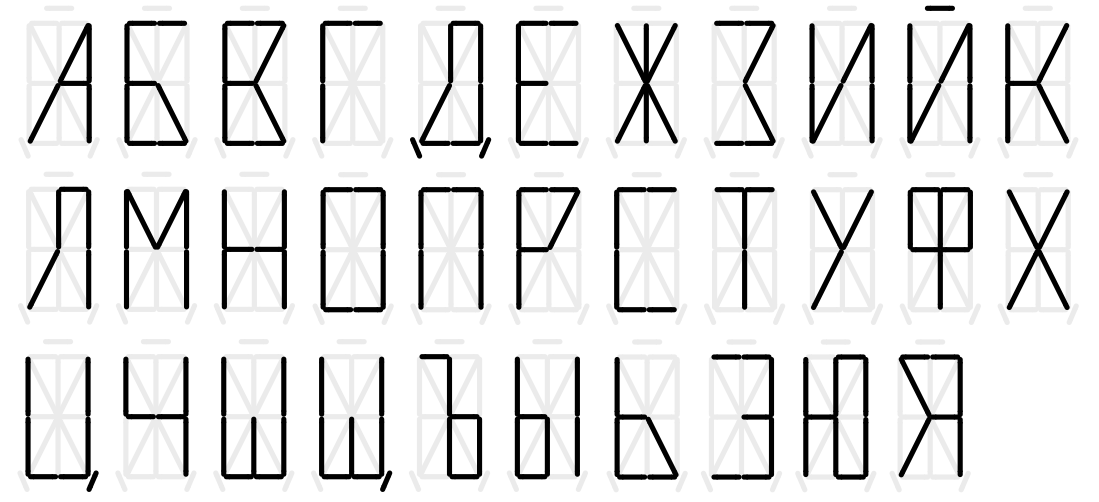
\includegraphics[width=6.2cm]{img/16seg} \pause \\ [0.25cm]
	Вспомним замеченное нами совпадение: \\
\begin{tabular}{ll}
\makecell[l]{{\footnotesize ЬР ЬЗ ЬВ СК СВ РЗ РВ РБ КЗ} \\
{\footnotesize КЕ КВ КБ ЗЕ ЗВ ЗБ ЕВ ГВ ВБ}} &
\makecell[l]{\tikz[scale=0.2]{
  \draw (-1.000000,2.000000) -- (-1.000000,0.000000);
  \draw (-1.000000,0.000000) -- (0.000000,0.000000);
  \draw (-1.000000,-2.000000) -- (-1.000000,0.000000);
  \draw (1.000000,-2.000000) -- (0.000000,0.000000);
  \draw (-1.000000,-2.000000) -- (0.000000,-2.000000);
  \draw (0.000000,-2.000000) -- (1.000000,-2.000000);
  \draw (-1.000000,2.000000) -- (0.000000,2.000000);
  \draw (0.000000,2.000000) -- (1.000000,2.000000);
  \draw (1.000000,2.000000) -- (0.000000,0.000000);
}}
\end{tabular}} & \pause \makecell[c]{
\includegraphics[width=6.5cm]{img/allex}}
\end{tabular} \end{frame}